\documentclass[tikz,border=0pt]{standalone}
\usepackage[american]{circuitikz}
\usetikzlibrary{arrows.meta,calc,positioning,decorations.pathmorphing,patterns}
\definecolor{zyloTeal}{HTML}{174A5B}
\definecolor{zyloTealTwo}{HTML}{246B7A}
\definecolor{zyloInk}{HTML}{1F2933}
\definecolor{zyloSoft}{HTML}{EAF4F4}
\definecolor{zyloPaper}{HTML}{F8FAFB}
\definecolor{zyloLine}{HTML}{44606B}
\definecolor{zyloOrange}{HTML}{D97706}
\begin{document}
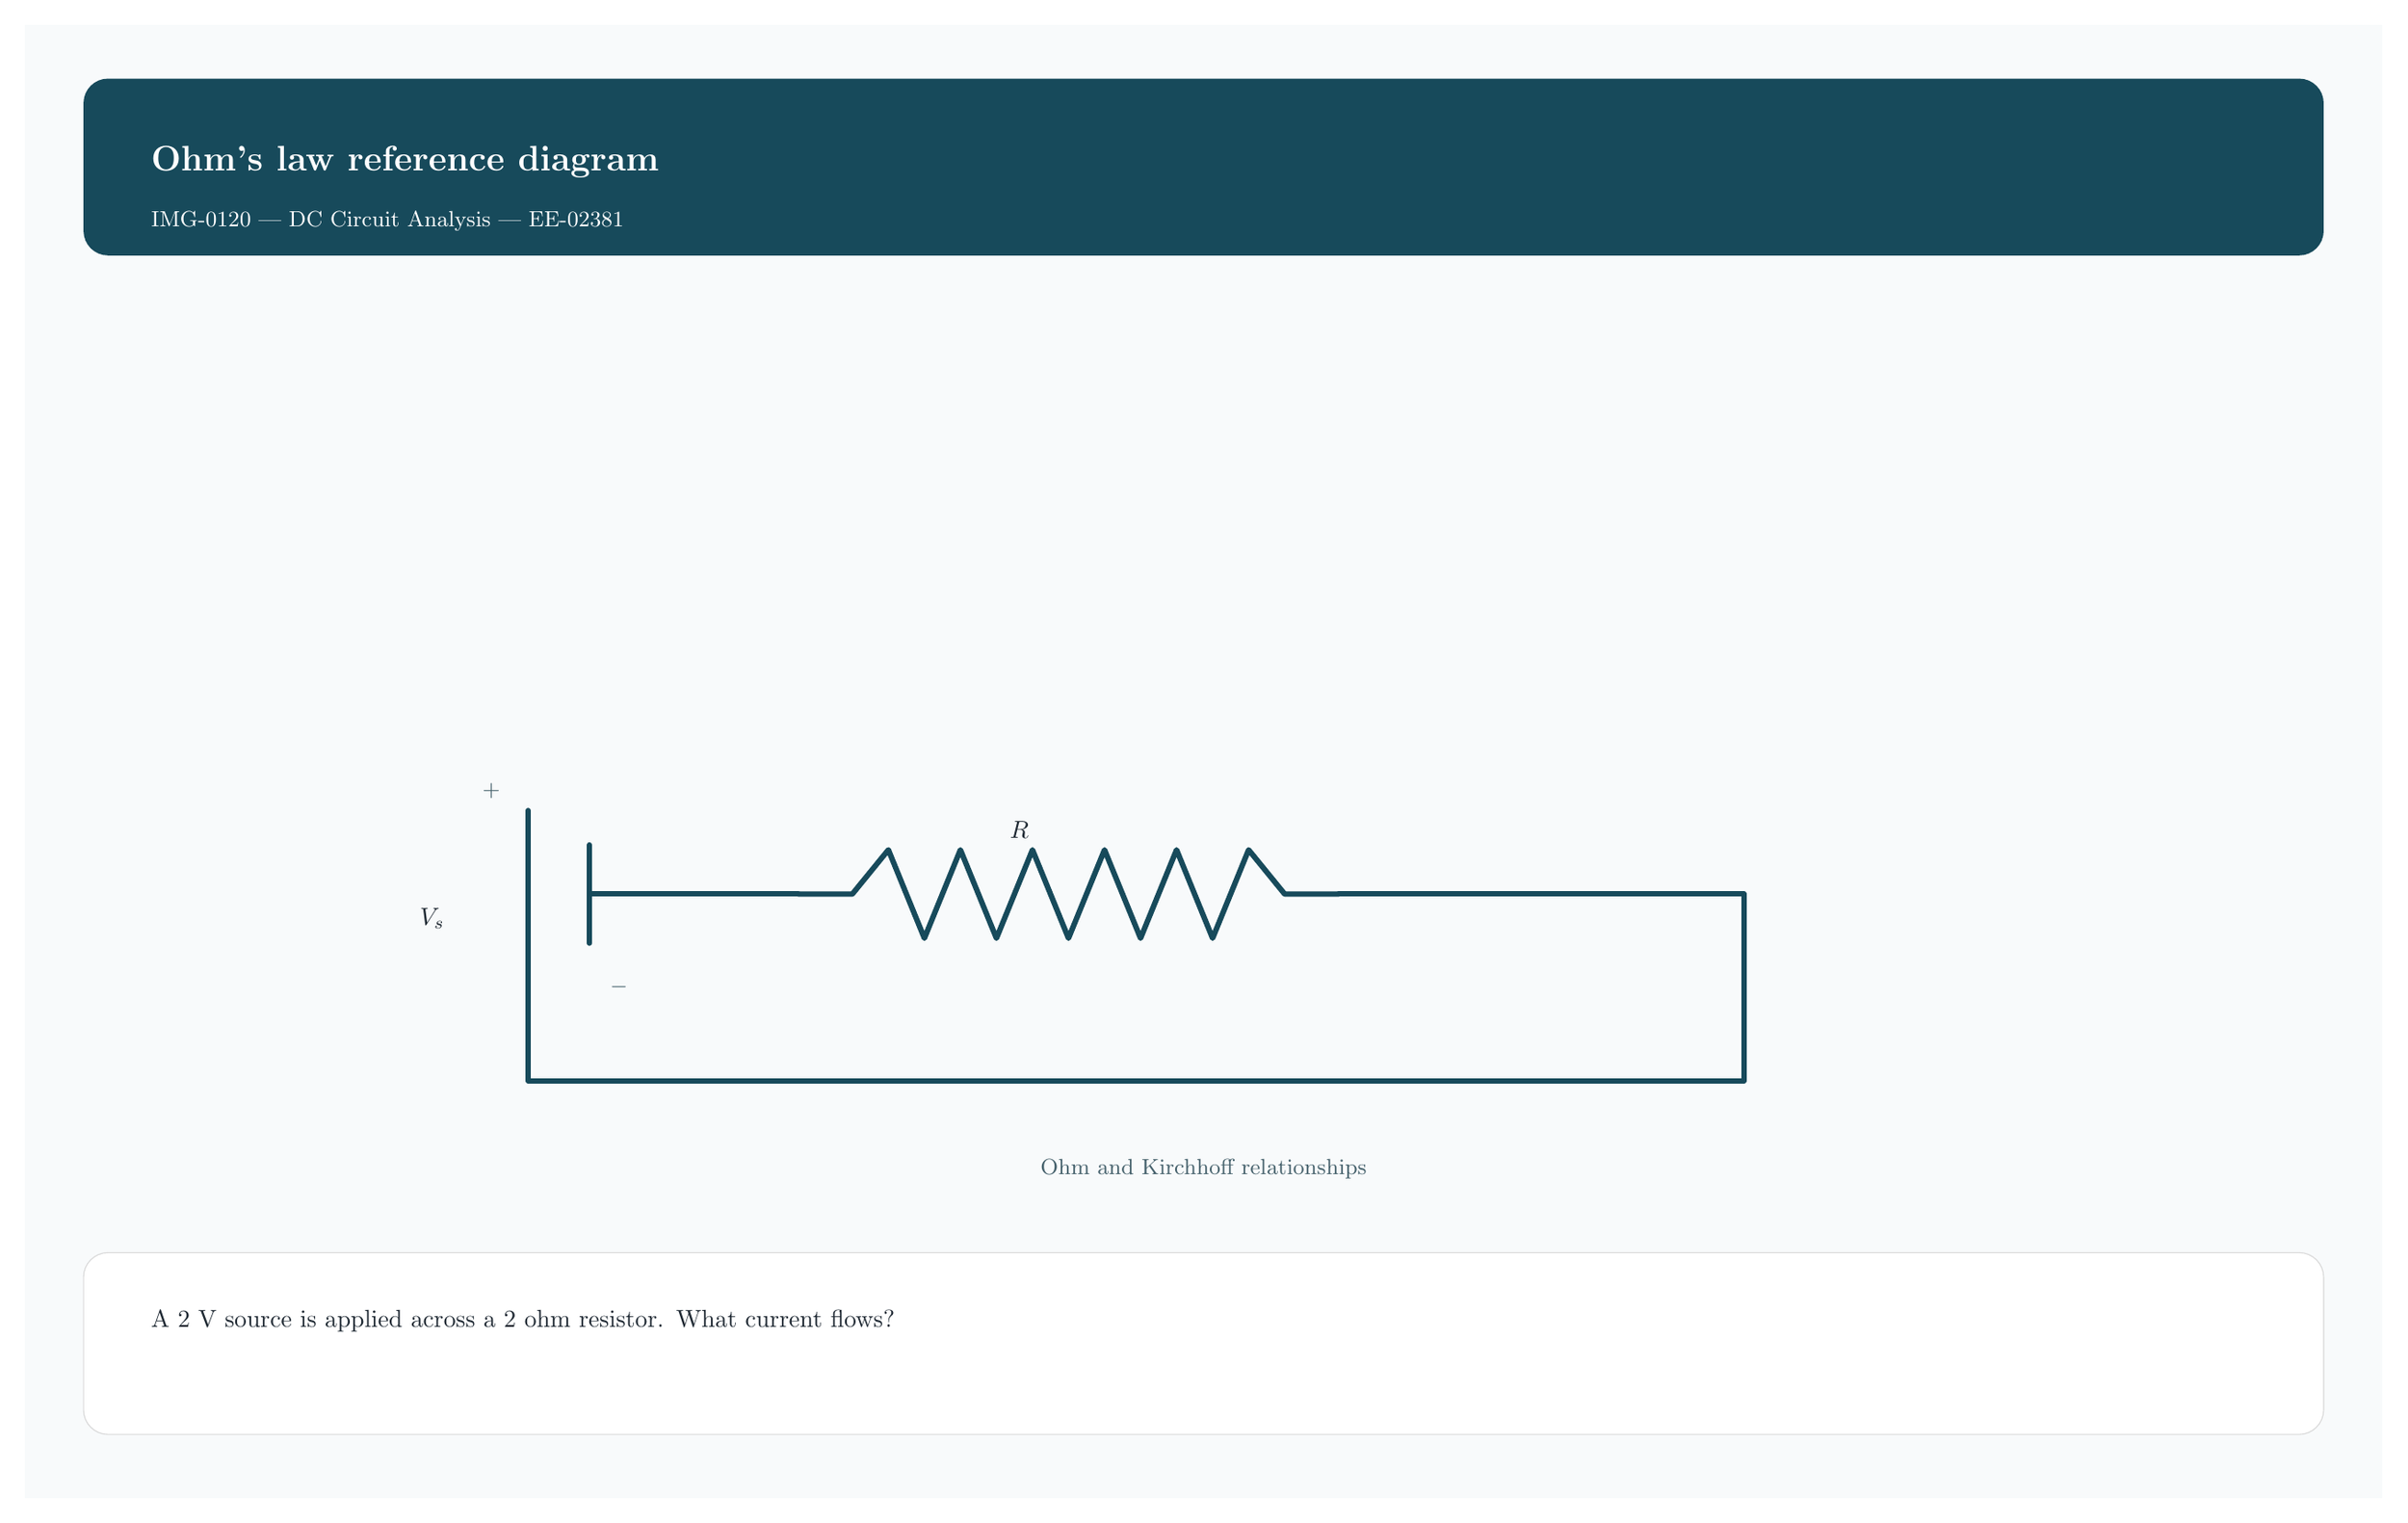
\begin{tikzpicture}[x=1pt,y=-1pt,>=Latex,line cap=round,line join=round]
\path[fill=zyloPaper] (0,0) rectangle (960,600);
\path[fill=zyloTeal,rounded corners=10pt] (24,22) rectangle (936,94);
\node[anchor=west,text=white,font=\bfseries\Large] at (48,56) {Ohm's law reference diagram};
\node[anchor=west,text=white!82,font=\small] at (48,80) {IMG-0120 | DC Circuit Analysis | EE-02381};
\tikzset{wire/.style={draw=zyloTeal,line width=2.2pt},thinwire/.style={draw=zyloLine,line width=1.35pt},accent/.style={draw=zyloOrange,line width=2.2pt},box/.style={draw=zyloTealTwo,fill=zyloSoft,line width=1.5pt,rounded corners=8pt}}
\draw[wire] (205,320) -- (205,388); \draw[wire] (230,334) -- (230,374);
\node[font=\small,text=zyloLine] at (190,312) {$+$}; \node[font=\small,text=zyloLine] at (242,392) {$-$};
\draw[wire] (230,354) -- (315,354);
\draw[wire] (315,354) -- (337,354) -- (337,354) -- (351.667,336) -- (366.333,372) -- (381,336) -- (395.667,372) -- (410.333,336) -- (425,372) -- (439.667,336) -- (454.333,372) -- (469,336) -- (483.667,372) -- (498.333,336) -- (513,354) -- (535,354);
\draw[wire] (535,354) -- (700,354) -- (700,430) -- (205,430) -- (205,388);
\node[text=zyloInk] at (405,328) {$R$}; \node[text=zyloInk] at (166,364) {$V_s$};
\node[font=\small,text=zyloLine] at (480,466) {Ohm and Kirchhoff relationships};
\path[draw=black!15,fill=white,rounded corners=10pt] (24,500) rectangle (936,574);
\node[anchor=west,text width=860pt,align=left,text=zyloInk,font=\normalsize] at (48,528) {A 2 V source is applied across a 2 ohm resistor. What current flows?};
\end{tikzpicture}
\end{document}
